This chapter presents an overview of our proposed architecture represented through a diagram. We also present the experimental design and the evaluation metrics that we will employ to evaluate the performance of our method. The information presented below is tentative and can be subject to change if a better approach is identified/discovered along the course of the project.

\section{Architecture Design}
\subsection{Proposed System Model}
The proposed system model will begin with the assumption that the data has been 
processed and filtered so as to reduce the noise within the data and process it 
according to the database compilation pipeline in Figure~\ref{fig: data_pipelinediag}. The dataset will contain the IDs and gene names of the proteins 
in each protein pair as well as their interaction score. This will then be used to 
create a PPI network object that can then be used in N base clustering algorithms to 
generate clusters. 

These base clustering algorithms will include the Direct k-way 
partitioning and multilevel k-level partitioning as described in Section~\ref{sec: 
ensemble framework}. After obtaining clusters we will then proceed to the core of the
ensemble framework. We will purify these clusters, prune them and apply principle component analysis (PCA) on the clusters. The clusters will also be turned into weighted graphs by adding weights after the purification block. The weighted graphs and the PCA together will then be used for agglomerate clustering which will give us out final cluster outputs which will be tested against our evaluation metrics.

A high level representation of the proposed system model can be seen in Figure~\ref{fig: systemdiag}.
\begin{figure}[h!]
    \centering
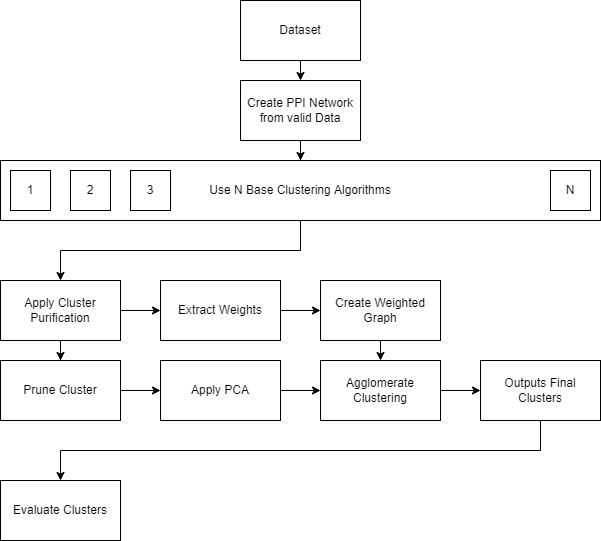
\includegraphics[scale=0.7]{Final-Report-Kavish-1/system_diagram (1).png}
\caption{Proposed System Diagram}
\label{fig: systemdiag}
\end{figure}

% \begin{enumerate}
% \item{Hypothesis}
% \item{Method}
% \item{Results}
% \item{Limitations of Methodology}
% \end{enumerate}

\section{Experimental Design \& Evaluation Metrics}
Since the problem of identifying protein complexes essentially boils down to a classification 
problem, where we are identifying known protein complexes (subgraphs) from a sea of candidate 
subgraphs. Therefore, after we obtain our final result, we can use a testing set generated from 
preexisting protein complex databases to evaluate our result. We will use the evaluation metrics 
that are generally used for classification problems. These include: 
\begin{enumerate}
\item{Precision \& Recall}: Precision is the fraction of relevant complexes among identified complexes while recall is the fraction of relevant complexes that were identified. Mathematically, they are computed as:
\[\text{Precision } = \frac{\{p \; | \; p \in P \; \wedge \; \exists r \in R, p \text{ matches } r\}}{|P|}\]
\[\text{Recall } = \frac{\{r \; | \; r \in R \; \land \; \exists p \in P, \; r \text{ matches } p\}}{|R|}\]

\item{$F$-Measure}:
The $F$-measure or $F$-score is calculated using precision and recall. More specifically, we will use the $F_1$ 
score to evaluate the performance of our method. The $F_1$ score is the harmonic mean of precision and recall and is given as:

\[F \text{ measure } = \frac{2 \cdot \text{Precision} \cdot \text{Recall}}{\text{Precision } + \text{ Recall}}\]

\item{Confusion Matrix}: We can create a confusion matrix $T$ from $n$ reference protein complexes and $m$ identified clusters:
\[T = \begin{bmatrix}
t_{1,1} & \ldots & t_{1,m} \\ 
\vdots & \ddots & \vdots \\ 
t_{1,n} & \ldots & t_{n,m}  
\end{bmatrix}\]
where $t_{i,j}$ indicates the number of proteins that the $i$-th known protein complex and the 
$j$-th cluster have in common. Using the confusion matrix, we can generate three other useful metrics:
\begin{itemize}
    \item Sensitivity (Sn) can be computed as:
    \[\text{Sn } = \frac{\sum_{i=1}^n \max_j{t_{ij}}}{f}\]
    \item Positive Predictive Value (PPV) is given as:
    \[\text{PPV } = \frac{\sum_{j=1}^m \max_i{t_{ij}}}{\sum_{j=1}^m \; \sum_{i=1}^n t_{ij}}\]
    \item Accuracy (Acc) can be computed using:
    \[\text{Acc } = \sqrt{\text{Sn} \times \text{PPV}}\]
\end{itemize}
\end{enumerate}
